\documentclass[]{article}
\usepackage{amssymb,amsmath}
\usepackage{ifxetex,ifluatex}
\ifxetex
  \usepackage{fontspec,xltxtra,xunicode}
  \defaultfontfeatures{Mapping=tex-text,Scale=MatchLowercase}
\else
  \ifluatex
    \usepackage{fontspec}
    \defaultfontfeatures{Mapping=tex-text,Scale=MatchLowercase}
  \else
    \usepackage[utf8]{inputenc}
  \fi
\fi
\usepackage{ctable}
\usepackage{float} % provides the H option for float placement
\usepackage{graphicx}
% We will generate all images so they have a width \maxwidth. This means
% that they will get their normal width if they fit onto the page, but
% are scaled down if they would overflow the margins.
\makeatletter
\def\maxwidth{\ifdim\Gin@nat@width>\linewidth\linewidth
\else\Gin@nat@width\fi}
\makeatother
\let\Oldincludegraphics\includegraphics
\renewcommand{\includegraphics}[1]{\Oldincludegraphics[width=\maxwidth]{#1}}
\ifxetex
  \usepackage[setpagesize=false, % page size defined by xetex
              unicode=false, % unicode breaks when used with xetex
              xetex,
              colorlinks=true,
              linkcolor=blue]{hyperref}
\else
  \usepackage[unicode=true,
              colorlinks=true,
              linkcolor=blue]{hyperref}
\fi
\hypersetup{breaklinks=true, pdfborder={0 0 0}}
\newcommand{\textsubscr}[1]{\ensuremath{_{\scriptsize\textrm{#1}}}}
\setlength{\parindent}{0pt}
\setlength{\parskip}{6pt plus 2pt minus 1pt}
\setlength{\emergencystretch}{3em}  % prevent overfull lines
\setcounter{secnumdepth}{0}

\title{Descriptive statistics}
\author{Rapport package team @ https://github.com/aL3xa/rapport}
\date{2011-04-26 20:25 CET}

\begin{document}
\maketitle

\subsection{Description}

This template will return descriptive statistics of numerical or
frequency tables of categorical variables.

\subsection{\emph{gender} (``Gender'')}

The dataset has \emph{709} observations with \emph{673} valid values
(missing: \emph{36}) in \emph{gender} (``Gender''), which seems to be a
qualitative variable.

\subsubsection{Base statistics}

\ctable[pos = H, center, botcap]{lllll}
{% notes
}
 & \textbf{Cumul.
N} & \textbf{Cumul. \%}
\ML
male & 410 & 60.9212 & 410 & 60.9212
\\\noalign{\medskip}
female & 263 & 39.0788 & 673 & 100
\\\noalign{\medskip}
Total & 673 & 100 & 673 & 100
\LL
}

\subsubsection{Barplot}

\href{3a46554ee29cd4dfe45dda5016464658-hires.png}{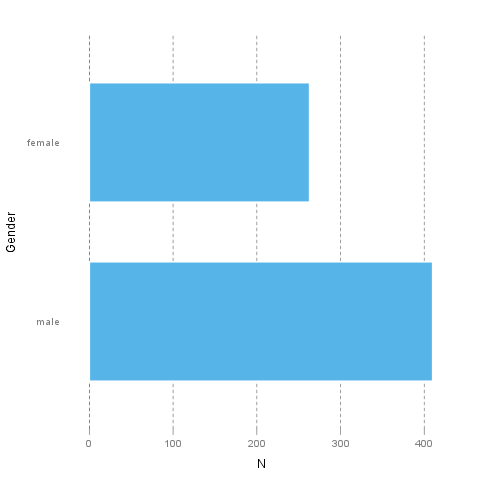
\includegraphics{3a46554ee29cd4dfe45dda5016464658.png}}

It seems that the highest value is \emph{2} which is exactly 2 times
higher than the smallest value (\emph{1}).

The most frequent value is \emph{male}.

\subsection{\emph{age} (``Age'')}

The dataset has \emph{709} observations with \emph{677} valid values
(missing: \emph{32}) in \emph{age} (``Age''), which seems to be a
quantitative variable.

\subsubsection{Base statistics}

\ctable[pos = H, center, botcap]{llll}
{% notes
}
{% rows
\FL
\textbf{Variable} & \textbf{mean} & \textbf{sd} & \textbf{var}
\ML
Age & 24.5731 & 6.8491 & 46.9107
\LL
}

\subsubsection{Histogram}

\href{4f025d440bf35d40e21208e8b0c58b77-hires.png}{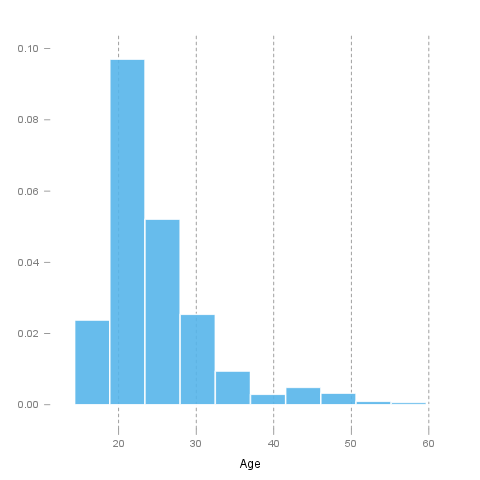
\includegraphics{4f025d440bf35d40e21208e8b0c58b77.png}}

It seems that the highest value is \emph{58} which is exactly 3.625
times higher than the smallest value (\emph{16}).

The standard deviation is \emph{6.8491} (variance: \emph{46.9107}). The
expected value is around \emph{24.5731}, somewhere between
\emph{24.0572} and \emph{25.0891} with the standard error of
\emph{0.2632}.

If we suppose that \emph{Age} is not near to a normal distribution
(test: see below, skewness: \emph{1.9296}, kurtosis: \emph{7.4851}),
checking the median (\emph{23}) might be a better option instead of the
mean. The interquartile range (\emph{6}) measures the statistics
dispersion of the variable (similar to standard deviation) based on
median.

\subsubsection{Normality tests}

\paragraph{Introduction}

In statistics, \emph{normality} refers to an assumption that the
distribution of a random variable follows \emph{normal}
(\emph{Gaussian}) distribution. Because of its bell-like shape, it's
also known as the \emph{``bell curve''}. The formula for \emph{normal
distribution} is:

\[f(x) = \frac{1}{\sqrt{2\pi{}\sigma{}^2}} e^{-\frac{(x-\mu{})^2}{2\sigma{}^2}}\]

\emph{Normal distribution} belongs to a \emph{location-scale family} of
distributions, as it's defined two parameters:

\begin{itemize}
\item
  \emph{μ} - \emph{mean} or \emph{expectation} (location parameter)
\item
  \emph{σ\textsuperscript{2}} - \emph{variance} (scale parameter)
\end{itemize}
\href{806ea97c59e1a12d4acae4968957aaa9-hires.png}{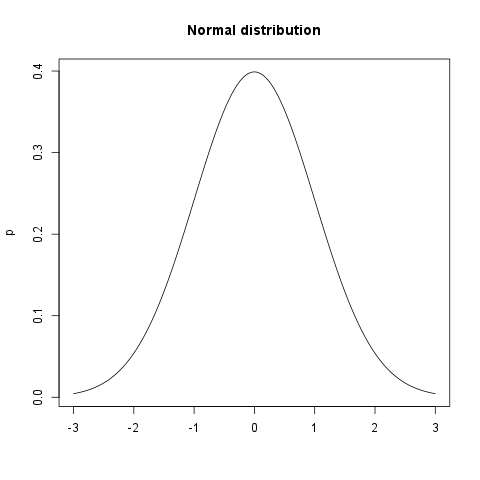
\includegraphics{806ea97c59e1a12d4acae4968957aaa9.png}}

\paragraph{Normality Tests}

\subparagraph{Overview}

Various hypothesis tests can be applied in order to test if the
distribution of given random variable violates normality assumption.
These procedures test the H\textsubscr{0} that provided variable's
distribution is \emph{normal}. At this point only few such tests will be
covered: the ones that are available in \texttt{stats} package (which
comes bundled with default R installation) and \texttt{nortest} package
that is
\href{http://cran.r-project.org/web/packages/nortest/index.html}{available}
on CRAN.

\begin{itemize}
\item
  \textbf{Shapiro-Wilk test} is a powerful normality test appropriate
  for small samples. In R, it's implemented in \texttt{shapiro.test}
  function available in \texttt{stats} package.
\item
  \textbf{Lilliefors test} is a modification of \emph{Kolmogorov-Smirnov
  test} appropriate for testing normality when parameters or normal
  distribution (\emph{μ}, \emph{σ\textsuperscript{2}}) are not known.
  \texttt{lillie.test} function is located in \texttt{nortest} package.
\item
  \textbf{Anderson-Darling test} is one of the most powerful normality
  tests as it will detect the most of departures from normality. You can
  find \texttt{ad.test} function in \texttt{nortest} package.
\item
  \textbf{Pearson Χ\textsuperscript{2} test} is another normality test
  which takes more ``traditional'' approach in normality testing.
  \texttt{pearson.test} is located in \texttt{nortest} package.
\end{itemize}
\subparagraph{Results}

Here you can see the results of applied normality tests (\emph{p-values}
less than 0.05 indicate significant discrepancies):

\emph{0.05}

So, let's draw some conclusions based on applied normality test:

\begin{itemize}
\item
  according to \emph{Shapiro-Wilk test}, the distribution of \emph{Age}
  is not normal.
\item
  based on \emph{Lilliefors test}, distribution of \emph{Age} is not
  normal
\item
  \emph{Anderson-Darling test} confirms violation of normality
  assumption
\item
  \emph{Pearson's Χ\textsuperscript{2} test} classifies the underlying
  distribution as non-normal
\end{itemize}
\paragraph{Diagnostic Plots}

There are various plots that can help you decide about the normality of
the distribution. Only a few most commonly used plots will be shown:
\emph{histogram}, \emph{Q-Q plot} and \emph{kernel density plot}.

\subparagraph{Histogram}

\emph{Histogram} was first introduced by \emph{Karl Pearson} and it's
probably the most popular plot for depicting the probability
distribution of a random variable. However, the decision depends on
number of bins, so it can sometimes be misleading. If the variable
distribution is normal, bins should resemble the ``bell-like'' shape.

\href{4f025d440bf35d40e21208e8b0c58b77-hires.png}{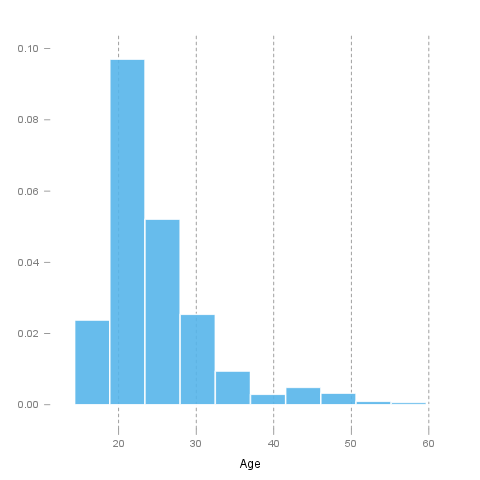
\includegraphics{4f025d440bf35d40e21208e8b0c58b77.png}}

\subparagraph{Q-Q Plot}

``Q'' in \emph{Q-Q plot} stands for \emph{quantile}, as this plot
compares empirical and theoretical distribution (in this case,
\emph{normal} distribution) by plotting their quantiles against each
other. For normal distribution, plotted dots should approximate a
``straight'', \texttt{x = y} line.

\href{131f20f388f78bd4863828d9fed8c35c-hires.png}{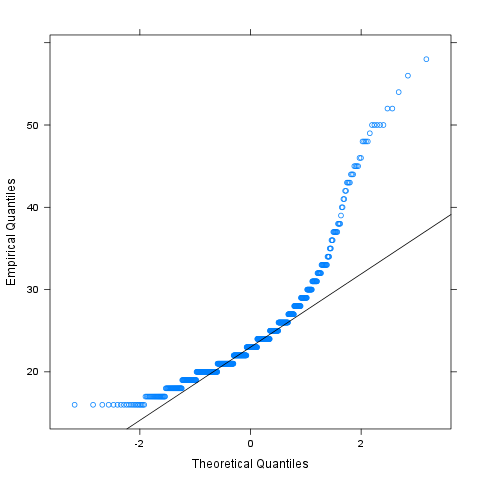
\includegraphics{131f20f388f78bd4863828d9fed8c35c.png}}

\subparagraph{Kernel Density Plot}

\emph{Kernel density plot} is a plot of smoothed \emph{empirical
distribution function}. As such, it provides good insight about the
shape of the distribution. For normal distributions, it should resemble
the well known ``bell shape''.

\href{d9ffb95307c560c15d33484c3a2d87f0-hires.png}{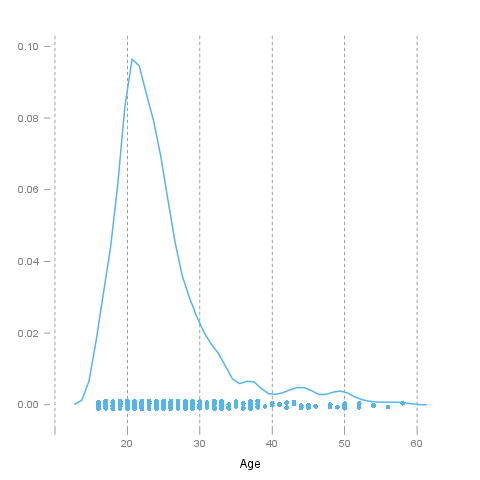
\includegraphics{d9ffb95307c560c15d33484c3a2d87f0.png}}

\subsection{Description}

This template will return descriptive statistics of numerical or
frequency tables of categorical variables.

\subsection{\emph{chatim} (``Chat \& IM usage'')}

The dataset has \emph{709} observations with \emph{669} valid values
(missing: \emph{40}) in \emph{chatim} (``Chat \& IM usage''), which
seems to be a qualitative variable.

\subsubsection{Base statistics}

\ctable[pos = H, center, botcap]{lllll}
{% notes
}
 & \textbf{Cumul.
N} & \textbf{Cumul. \%}
\ML
never & 60 & 8.9686 & 60 & 8.9686
\\\noalign{\medskip}
very rarely & 73 & 10.9118 & 133 & 19.8804
\\\noalign{\medskip}
rarely & 58 & 8.6697 & 191 & 28.5501
\\\noalign{\medskip}
sometimes & 113 & 16.8909 & 304 & 45.441
\\\noalign{\medskip}
often & 136 & 20.3288 & 440 & 65.7698
\\\noalign{\medskip}
very often & 88 & 13.154 & 528 & 78.9238
\\\noalign{\medskip}
always & 141 & 21.0762 & 669 & 100
\\\noalign{\medskip}
Total & 669 & 100 & 669 & 100
\LL
}

\subsubsection{Barplot}

\href{a3a825d8535e7c9b8a9d23cc8c1293b1-hires.png}{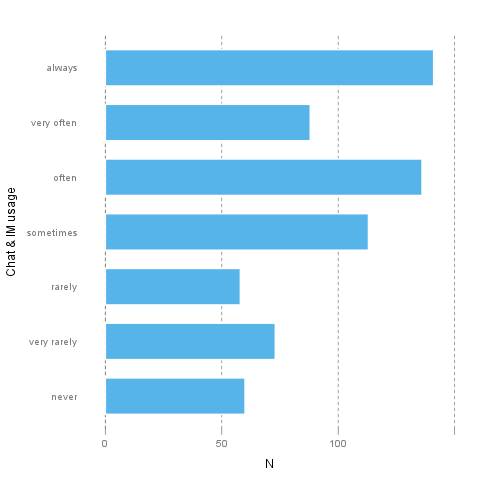
\includegraphics{a3a825d8535e7c9b8a9d23cc8c1293b1.png}}

It seems that the highest value is \emph{7} which is exactly 7 times
higher than the smallest value (\emph{1}).

The most frequent value is \emph{always}.

\subsection{\emph{game} (``On-line games usage'')}

The dataset has \emph{709} observations with \emph{677} valid values
(missing: \emph{32}) in \emph{game} (``On-line games usage''), which
seems to be a qualitative variable.

\subsubsection{Base statistics}

\ctable[pos = H, center, botcap]{lllll}
{% notes
}
 & \textbf{Cumul.
N} & \textbf{Cumul. \%}
\ML
never & 352 & 51.9941 & 352 & 51.9941
\\\noalign{\medskip}
very rarely & 128 & 18.9069 & 480 & 70.901
\\\noalign{\medskip}
rarely & 32 & 4.7267 & 512 & 75.6278
\\\noalign{\medskip}
sometimes & 60 & 8.8626 & 572 & 84.4904
\\\noalign{\medskip}
often & 37 & 5.4653 & 609 & 89.9557
\\\noalign{\medskip}
very often & 35 & 5.1699 & 644 & 95.1256
\\\noalign{\medskip}
always & 33 & 4.8744 & 677 & 100
\\\noalign{\medskip}
Total & 677 & 100 & 677 & 100
\LL
}

\subsubsection{Barplot}

\href{601bf73b7f424e34c795446ca73a1bac-hires.png}{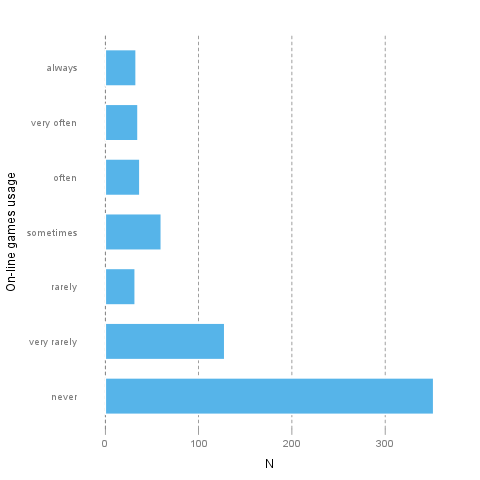
\includegraphics{601bf73b7f424e34c795446ca73a1bac.png}}

It seems that the highest value is \emph{7} which is exactly 7 times
higher than the smallest value (\emph{1}).

The most frequent value is \emph{never}.

\subsection{\emph{surf} (``Web surfing usage'')}

The dataset has \emph{709} observations with \emph{678} valid values
(missing: \emph{31}) in \emph{surf} (``Web surfing usage''), which seems
to be a qualitative variable.

\subsubsection{Base statistics}

\ctable[pos = H, center, botcap]{lllll}
{% notes
}
 & \textbf{Cumul.
N} & \textbf{Cumul. \%}
\ML
never & 17 & 2.5074 & 17 & 2.5074
\\\noalign{\medskip}
very rarely & 26 & 3.8348 & 43 & 6.3422
\\\noalign{\medskip}
rarely & 33 & 4.8673 & 76 & 11.2094
\\\noalign{\medskip}
sometimes & 107 & 15.7817 & 183 & 26.9912
\\\noalign{\medskip}
often & 158 & 23.3038 & 341 & 50.295
\\\noalign{\medskip}
very often & 142 & 20.944 & 483 & 71.2389
\\\noalign{\medskip}
always & 195 & 28.7611 & 678 & 100
\\\noalign{\medskip}
Total & 678 & 100 & 678 & 100
\LL
}

\subsubsection{Barplot}

\href{8b8013a5d21daf05463bf12edc7d6bfa-hires.png}{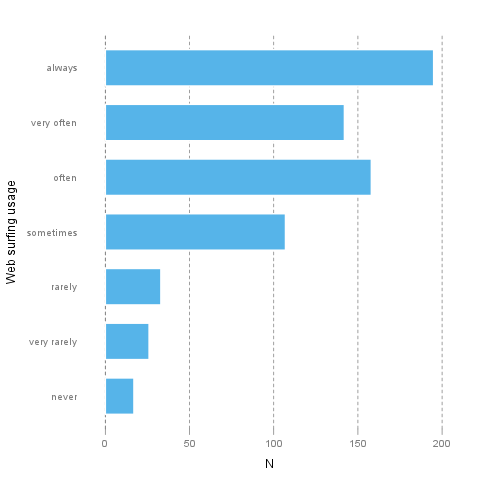
\includegraphics{8b8013a5d21daf05463bf12edc7d6bfa.png}}

It seems that the highest value is \emph{7} which is exactly 7 times
higher than the smallest value (\emph{1}).

The most frequent value is \emph{always}.

\subsection{\emph{email} (``Email usage'')}

The dataset has \emph{709} observations with \emph{672} valid values
(missing: \emph{37}) in \emph{email} (``Email usage''), which seems to
be a qualitative variable.

\subsubsection{Base statistics}

\ctable[pos = H, center, botcap]{lllll}
{% notes
}
 & \textbf{Cumul.
N} & \textbf{Cumul. \%}
\ML
never & 13 & 1.9345 & 13 & 1.9345
\\\noalign{\medskip}
very rarely & 36 & 5.3571 & 49 & 7.2917
\\\noalign{\medskip}
rarely & 46 & 6.8452 & 95 & 14.1369
\\\noalign{\medskip}
sometimes & 87 & 12.9464 & 182 & 27.0833
\\\noalign{\medskip}
often & 123 & 18.3036 & 305 & 45.3869
\\\noalign{\medskip}
very often & 108 & 16.0714 & 413 & 61.4583
\\\noalign{\medskip}
always & 259 & 38.5417 & 672 & 100
\\\noalign{\medskip}
Total & 672 & 100 & 672 & 100
\LL
}

\subsubsection{Barplot}

\href{7d530054059115b70f8098f2e3ff6c81-hires.png}{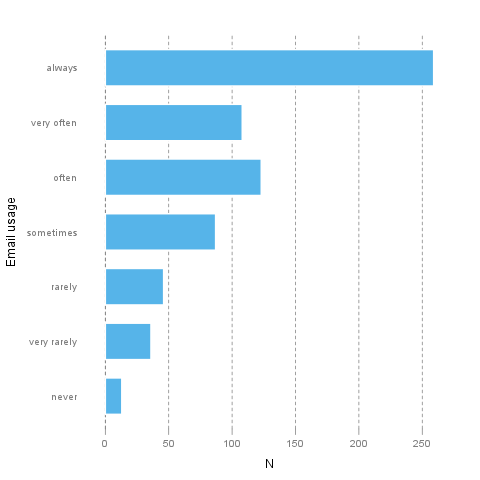
\includegraphics{7d530054059115b70f8098f2e3ff6c81.png}}

It seems that the highest value is \emph{7} which is exactly 7 times
higher than the smallest value (\emph{1}).

The most frequent value is \emph{always}.

\subsection{\emph{download} (``Download usage'')}

The dataset has \emph{709} observations with \emph{677} valid values
(missing: \emph{32}) in \emph{download} (``Download usage''), which
seems to be a qualitative variable.

\subsubsection{Base statistics}

\ctable[pos = H, center, botcap]{lllll}
{% notes
}
 & \textbf{Cumul.
N} & \textbf{Cumul. \%}
\ML
never & 11 & 1.6248 & 11 & 1.6248
\\\noalign{\medskip}
very rarely & 28 & 4.1359 & 39 & 5.7607
\\\noalign{\medskip}
rarely & 29 & 4.2836 & 68 & 10.0443
\\\noalign{\medskip}
sometimes & 80 & 11.8168 & 148 & 21.8612
\\\noalign{\medskip}
often & 124 & 18.3161 & 272 & 40.1773
\\\noalign{\medskip}
very often & 160 & 23.6337 & 432 & 63.8109
\\\noalign{\medskip}
always & 245 & 36.1891 & 677 & 100
\\\noalign{\medskip}
Total & 677 & 100 & 677 & 100
\LL
}

\subsubsection{Barplot}

\href{c5c68401731dd8623c3bac532d4f93b1-hires.png}{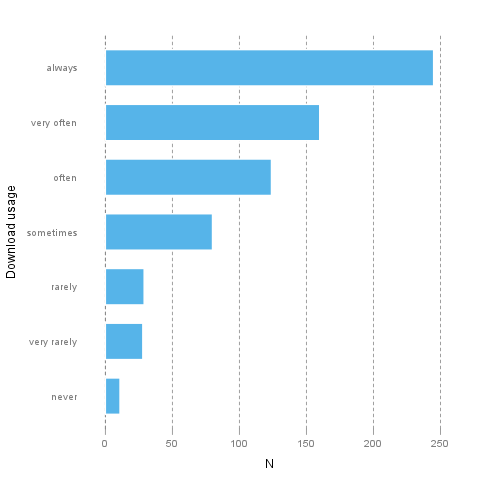
\includegraphics{c5c68401731dd8623c3bac532d4f93b1.png}}

It seems that the highest value is \emph{7} which is exactly 7 times
higher than the smallest value (\emph{1}).

The most frequent value is \emph{always}.

\subsection{\emph{forum} (``Web forums usage'')}

The dataset has \emph{709} observations with \emph{673} valid values
(missing: \emph{36}) in \emph{forum} (``Web forums usage''), which seems
to be a qualitative variable.

\subsubsection{Base statistics}

\ctable[pos = H, center, botcap]{lllll}
{% notes
}
 & \textbf{Cumul.
N} & \textbf{Cumul. \%}
\ML
never & 76 & 11.2927 & 76 & 11.2927
\\\noalign{\medskip}
very rarely & 80 & 11.8871 & 156 & 23.1798
\\\noalign{\medskip}
rarely & 72 & 10.6984 & 228 & 33.8782
\\\noalign{\medskip}
sometimes & 111 & 16.4933 & 339 & 50.3715
\\\noalign{\medskip}
often & 109 & 16.1961 & 448 & 66.5676
\\\noalign{\medskip}
very often & 119 & 17.682 & 567 & 84.2496
\\\noalign{\medskip}
always & 106 & 15.7504 & 673 & 100
\\\noalign{\medskip}
Total & 673 & 100 & 673 & 100
\LL
}

\subsubsection{Barplot}

\href{e866a67bba62e7f5cbe93b184599019f-hires.png}{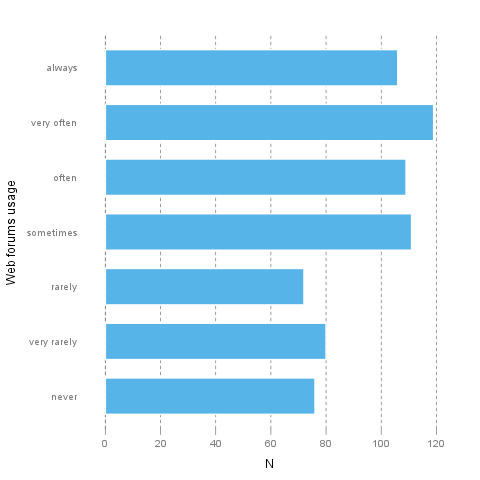
\includegraphics{e866a67bba62e7f5cbe93b184599019f.png}}

It seems that the highest value is \emph{7} which is exactly 7 times
higher than the smallest value (\emph{1}).

The most frequent value is \emph{very often}.

\subsection{\emph{socnet} (``Social networks usage'')}

The dataset has \emph{709} observations with \emph{678} valid values
(missing: \emph{31}) in \emph{socnet} (``Social networks usage''), which
seems to be a qualitative variable.

\subsubsection{Base statistics}

\ctable[pos = H, center, botcap]{lllll}
{% notes
}
 & \textbf{Cumul.
N} & \textbf{Cumul. \%}
\ML
never & 208 & 30.6785 & 208 & 30.6785
\\\noalign{\medskip}
very rarely & 102 & 15.0442 & 310 & 45.7227
\\\noalign{\medskip}
rarely & 57 & 8.4071 & 367 & 54.1298
\\\noalign{\medskip}
sometimes & 87 & 12.8319 & 454 & 66.9617
\\\noalign{\medskip}
often & 79 & 11.6519 & 533 & 78.6136
\\\noalign{\medskip}
very often & 80 & 11.7994 & 613 & 90.413
\\\noalign{\medskip}
always & 65 & 9.587 & 678 & 100
\\\noalign{\medskip}
Total & 678 & 100 & 678 & 100
\LL
}

\subsubsection{Barplot}

\href{6619f2daf580503ce53708176cb0d83b-hires.png}{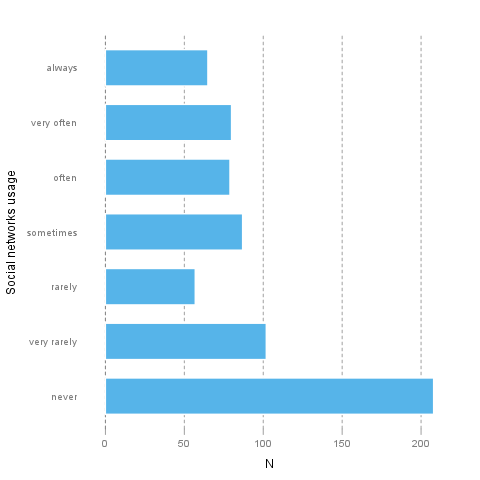
\includegraphics{6619f2daf580503ce53708176cb0d83b.png}}

It seems that the highest value is \emph{7} which is exactly 7 times
higher than the smallest value (\emph{1}).

The most frequent value is \emph{never}.

\subsection{\emph{xxx} (``Adult sites usage'')}

The dataset has \emph{709} observations with \emph{674} valid values
(missing: \emph{35}) in \emph{xxx} (``Adult sites usage''), which seems
to be a qualitative variable.

\subsubsection{Base statistics}

\ctable[pos = H, center, botcap]{lllll}
{% notes
}
 & \textbf{Cumul.
N} & \textbf{Cumul. \%}
\ML
never & 274 & 40.6528 & 274 & 40.6528
\\\noalign{\medskip}
very rarely & 124 & 18.3976 & 398 & 59.0504
\\\noalign{\medskip}
rarely & 52 & 7.7151 & 450 & 66.7656
\\\noalign{\medskip}
sometimes & 131 & 19.4362 & 581 & 86.2018
\\\noalign{\medskip}
often & 46 & 6.8249 & 627 & 93.0267
\\\noalign{\medskip}
very often & 28 & 4.1543 & 655 & 97.181
\\\noalign{\medskip}
always & 19 & 2.819 & 674 & 100
\\\noalign{\medskip}
Total & 674 & 100 & 674 & 100
\LL
}

\subsubsection{Barplot}

\href{cbda2b116fe3f7095f2997068f945424-hires.png}{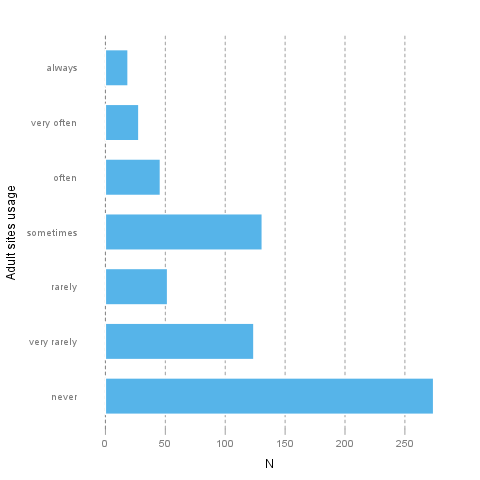
\includegraphics{cbda2b116fe3f7095f2997068f945424.png}}

It seems that the highest value is \emph{7} which is exactly 7 times
higher than the smallest value (\emph{1}).

The most frequent value is \emph{never}.

\subsection{Description}

This template will return descriptive statistics of numerical or
frequency tables of categorical variables.

\subsection{\emph{hp}}

The dataset has \emph{32} observations with \emph{32} valid values
(missing: \emph{0}) in \emph{hp}, which seems to be a quantitative
variable.

\subsubsection{Base statistics}

\ctable[pos = H, center, botcap]{llll}
{% notes
}
{% rows
\FL
\textbf{Variable} & \textbf{mean} & \textbf{sd} & \textbf{var}
\ML
hp & 146.6875 & 68.5629 & 4700.8669
\LL
}

\subsubsection{Histogram}

\href{78517cde85fc1ba06a3513dd17e567da-hires.png}{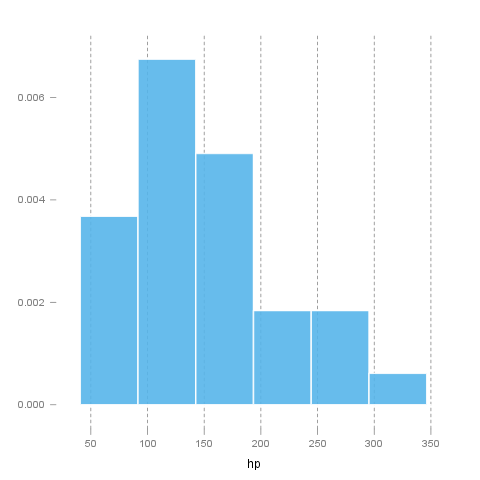
\includegraphics{78517cde85fc1ba06a3513dd17e567da.png}}

It seems that the highest value is \emph{335} which is exactly 6.4423
times higher than the smallest value (\emph{52}).

The standard deviation is \emph{68.5629} (variance: \emph{4700.8669}).
The expected value is around \emph{146.6875}, somewhere between
\emph{122.9317} and \emph{170.4433} with the standard error of
\emph{12.1203}.

If we suppose that \emph{hp} is not near to a normal distribution (test:
see below, skewness: \emph{0.7614}, kurtosis: \emph{3.0522}), checking
the median (\emph{123}) might be a better option instead of the mean.
The interquartile range (\emph{83.5}) measures the statistics dispersion
of the variable (similar to standard deviation) based on median.

\subsubsection{Normality tests}

\paragraph{Introduction}

In statistics, \emph{normality} refers to an assumption that the
distribution of a random variable follows \emph{normal}
(\emph{Gaussian}) distribution. Because of its bell-like shape, it's
also known as the \emph{``bell curve''}. The formula for \emph{normal
distribution} is:

\[f(x) = \frac{1}{\sqrt{2\pi{}\sigma{}^2}} e^{-\frac{(x-\mu{})^2}{2\sigma{}^2}}\]

\emph{Normal distribution} belongs to a \emph{location-scale family} of
distributions, as it's defined two parameters:

\begin{itemize}
\item
  \emph{μ} - \emph{mean} or \emph{expectation} (location parameter)
\item
  \emph{σ\textsuperscript{2}} - \emph{variance} (scale parameter)
\end{itemize}
\href{806ea97c59e1a12d4acae4968957aaa9-hires.png}{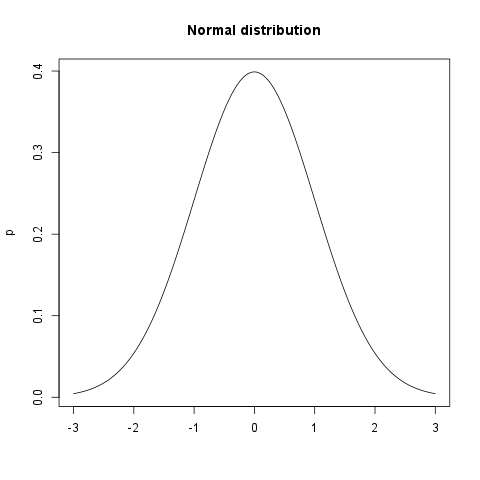
\includegraphics{806ea97c59e1a12d4acae4968957aaa9.png}}

\paragraph{Normality Tests}

\subparagraph{Overview}

Various hypothesis tests can be applied in order to test if the
distribution of given random variable violates normality assumption.
These procedures test the H\textsubscr{0} that provided variable's
distribution is \emph{normal}. At this point only few such tests will be
covered: the ones that are available in \texttt{stats} package (which
comes bundled with default R installation) and \texttt{nortest} package
that is
\href{http://cran.r-project.org/web/packages/nortest/index.html}{available}
on CRAN.

\begin{itemize}
\item
  \textbf{Shapiro-Wilk test} is a powerful normality test appropriate
  for small samples. In R, it's implemented in \texttt{shapiro.test}
  function available in \texttt{stats} package.
\item
  \textbf{Lilliefors test} is a modification of \emph{Kolmogorov-Smirnov
  test} appropriate for testing normality when parameters or normal
  distribution (\emph{μ}, \emph{σ\textsuperscript{2}}) are not known.
  \texttt{lillie.test} function is located in \texttt{nortest} package.
\item
  \textbf{Anderson-Darling test} is one of the most powerful normality
  tests as it will detect the most of departures from normality. You can
  find \texttt{ad.test} function in \texttt{nortest} package.
\item
  \textbf{Pearson Χ\textsuperscript{2} test} is another normality test
  which takes more ``traditional'' approach in normality testing.
  \texttt{pearson.test} is located in \texttt{nortest} package.
\end{itemize}
\subparagraph{Results}

Here you can see the results of applied normality tests (\emph{p-values}
less than 0.05 indicate significant discrepancies):

\emph{0.05}

So, let's draw some conclusions based on applied normality test:

\begin{itemize}
\item
  according to \emph{Shapiro-Wilk test}, the distribution of \emph{hp}
  is not normal.
\item
  based on \emph{Lilliefors test}, distribution of \emph{hp} is not
  normal
\item
  \emph{Anderson-Darling test} confirms normality assumption
\item
  \emph{Pearson's Χ\textsuperscript{2} test} classifies the underlying
  distribution as non-normal
\end{itemize}
\paragraph{Diagnostic Plots}

There are various plots that can help you decide about the normality of
the distribution. Only a few most commonly used plots will be shown:
\emph{histogram}, \emph{Q-Q plot} and \emph{kernel density plot}.

\subparagraph{Histogram}

\emph{Histogram} was first introduced by \emph{Karl Pearson} and it's
probably the most popular plot for depicting the probability
distribution of a random variable. However, the decision depends on
number of bins, so it can sometimes be misleading. If the variable
distribution is normal, bins should resemble the ``bell-like'' shape.

\href{78517cde85fc1ba06a3513dd17e567da-hires.png}{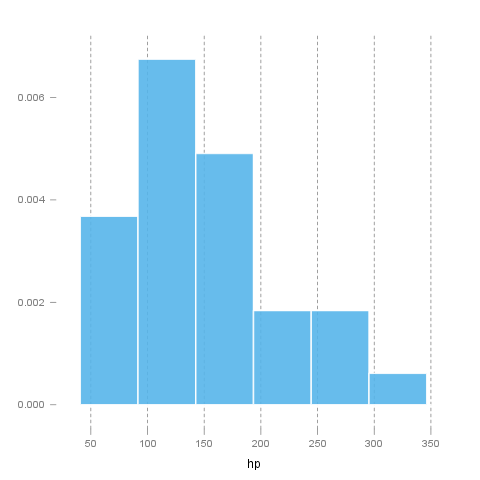
\includegraphics{78517cde85fc1ba06a3513dd17e567da.png}}

\subparagraph{Q-Q Plot}

``Q'' in \emph{Q-Q plot} stands for \emph{quantile}, as this plot
compares empirical and theoretical distribution (in this case,
\emph{normal} distribution) by plotting their quantiles against each
other. For normal distribution, plotted dots should approximate a
``straight'', \texttt{x = y} line.

\href{1cefec04e4451a937a5c6aa4dfdcb352-hires.png}{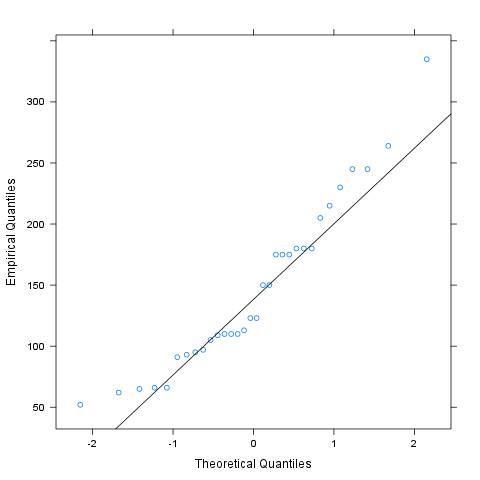
\includegraphics{1cefec04e4451a937a5c6aa4dfdcb352.png}}

\subparagraph{Kernel Density Plot}

\emph{Kernel density plot} is a plot of smoothed \emph{empirical
distribution function}. As such, it provides good insight about the
shape of the distribution. For normal distributions, it should resemble
the well known ``bell shape''.

\href{6fabf9a1622d1251d1e917289ebb984a-hires.png}{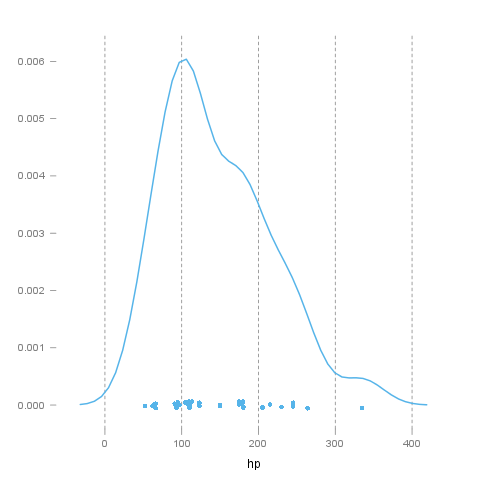
\includegraphics{6fabf9a1622d1251d1e917289ebb984a.png}}

\subsection{\emph{wt}}

The dataset has \emph{32} observations with \emph{32} valid values
(missing: \emph{0}) in \emph{wt}, which seems to be a quantitative
variable.

\subsubsection{Base statistics}

\ctable[pos = H, center, botcap]{llll}
{% notes
}
{% rows
\FL
\textbf{Variable} & \textbf{mean} & \textbf{sd} & \textbf{var}
\ML
wt & 3.2172 & 0.9785 & 0.9574
\LL
}

\subsubsection{Histogram}

\href{bf47295875cfa6d1667455a7d2721b19-hires.png}{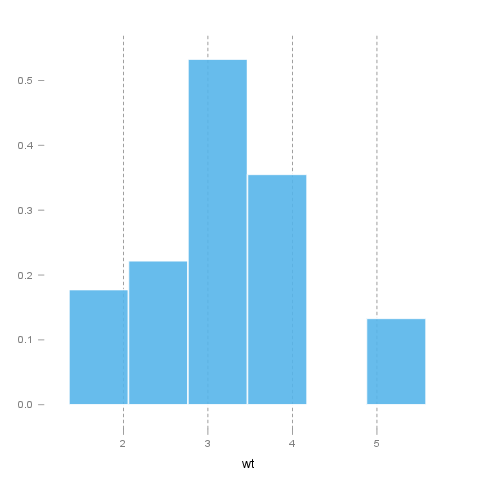
\includegraphics{bf47295875cfa6d1667455a7d2721b19.png}}

It seems that the highest value is \emph{5.424} which is exactly 3.5849
times higher than the smallest value (\emph{1.513}).

The standard deviation is \emph{0.9785} (variance: \emph{0.9574}). The
expected value is around \emph{3.2172}, somewhere between \emph{2.8782}
and \emph{3.5563} with the standard error of \emph{0.173}.

If we suppose that \emph{wt} is not near to a normal distribution (test:
see below, skewness: \emph{0.4438}, kurtosis: \emph{3.1725}), checking
the median (\emph{3.325}) might be a better option instead of the mean.
The interquartile range (\emph{1.0288}) measures the statistics
dispersion of the variable (similar to standard deviation) based on
median.

\subsubsection{Normality tests}

\paragraph{Introduction}

In statistics, \emph{normality} refers to an assumption that the
distribution of a random variable follows \emph{normal}
(\emph{Gaussian}) distribution. Because of its bell-like shape, it's
also known as the \emph{``bell curve''}. The formula for \emph{normal
distribution} is:

\[f(x) = \frac{1}{\sqrt{2\pi{}\sigma{}^2}} e^{-\frac{(x-\mu{})^2}{2\sigma{}^2}}\]

\emph{Normal distribution} belongs to a \emph{location-scale family} of
distributions, as it's defined two parameters:

\begin{itemize}
\item
  \emph{μ} - \emph{mean} or \emph{expectation} (location parameter)
\item
  \emph{σ\textsuperscript{2}} - \emph{variance} (scale parameter)
\end{itemize}
\href{806ea97c59e1a12d4acae4968957aaa9-hires.png}{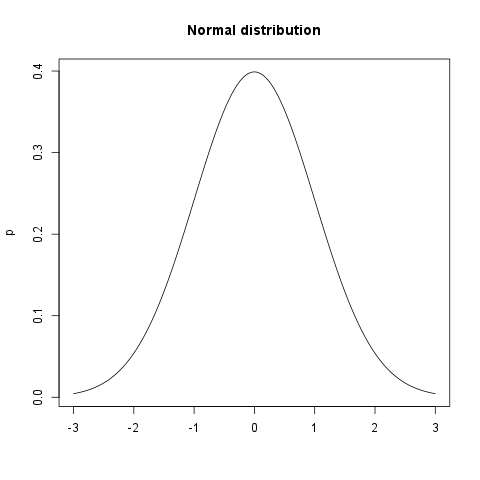
\includegraphics{806ea97c59e1a12d4acae4968957aaa9.png}}

\paragraph{Normality Tests}

\subparagraph{Overview}

Various hypothesis tests can be applied in order to test if the
distribution of given random variable violates normality assumption.
These procedures test the H\textsubscr{0} that provided variable's
distribution is \emph{normal}. At this point only few such tests will be
covered: the ones that are available in \texttt{stats} package (which
comes bundled with default R installation) and \texttt{nortest} package
that is
\href{http://cran.r-project.org/web/packages/nortest/index.html}{available}
on CRAN.

\begin{itemize}
\item
  \textbf{Shapiro-Wilk test} is a powerful normality test appropriate
  for small samples. In R, it's implemented in \texttt{shapiro.test}
  function available in \texttt{stats} package.
\item
  \textbf{Lilliefors test} is a modification of \emph{Kolmogorov-Smirnov
  test} appropriate for testing normality when parameters or normal
  distribution (\emph{μ}, \emph{σ\textsuperscript{2}}) are not known.
  \texttt{lillie.test} function is located in \texttt{nortest} package.
\item
  \textbf{Anderson-Darling test} is one of the most powerful normality
  tests as it will detect the most of departures from normality. You can
  find \texttt{ad.test} function in \texttt{nortest} package.
\item
  \textbf{Pearson Χ\textsuperscript{2} test} is another normality test
  which takes more ``traditional'' approach in normality testing.
  \texttt{pearson.test} is located in \texttt{nortest} package.
\end{itemize}
\subparagraph{Results}

Here you can see the results of applied normality tests (\emph{p-values}
less than 0.05 indicate significant discrepancies):

\emph{0.05}

So, let's draw some conclusions based on applied normality test:

\begin{itemize}
\item
  according to \emph{Shapiro-Wilk test}, the distribution of \emph{wt}
  is normal.
\item
  based on \emph{Lilliefors test}, distribution of \emph{wt} is not
  normal
\item
  \emph{Anderson-Darling test} confirms normality assumption
\item
  \emph{Pearson's Χ\textsuperscript{2} test} classifies the underlying
  distribution as non-normal
\end{itemize}
\paragraph{Diagnostic Plots}

There are various plots that can help you decide about the normality of
the distribution. Only a few most commonly used plots will be shown:
\emph{histogram}, \emph{Q-Q plot} and \emph{kernel density plot}.

\subparagraph{Histogram}

\emph{Histogram} was first introduced by \emph{Karl Pearson} and it's
probably the most popular plot for depicting the probability
distribution of a random variable. However, the decision depends on
number of bins, so it can sometimes be misleading. If the variable
distribution is normal, bins should resemble the ``bell-like'' shape.

\href{bf47295875cfa6d1667455a7d2721b19-hires.png}{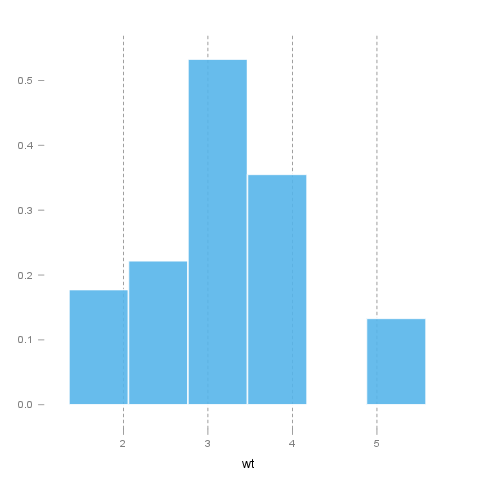
\includegraphics{bf47295875cfa6d1667455a7d2721b19.png}}

\subparagraph{Q-Q Plot}

``Q'' in \emph{Q-Q plot} stands for \emph{quantile}, as this plot
compares empirical and theoretical distribution (in this case,
\emph{normal} distribution) by plotting their quantiles against each
other. For normal distribution, plotted dots should approximate a
``straight'', \texttt{x = y} line.

\href{975387b3193e28fb08a85f37cb17f87e-hires.png}{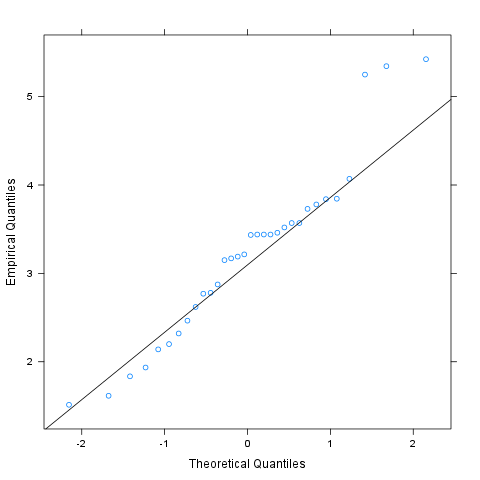
\includegraphics{975387b3193e28fb08a85f37cb17f87e.png}}

\subparagraph{Kernel Density Plot}

\emph{Kernel density plot} is a plot of smoothed \emph{empirical
distribution function}. As such, it provides good insight about the
shape of the distribution. For normal distributions, it should resemble
the well known ``bell shape''.

\href{68d781df2baa06f59e1f194c9b06ddac-hires.png}{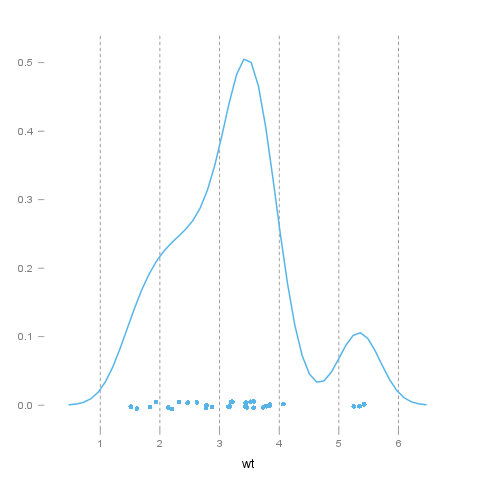
\includegraphics{68d781df2baa06f59e1f194c9b06ddac.png}}

\begin{center}\rule{3in}{0.4pt}\end{center}

This report was generated with \href{http://www.r-project.org/}{R}
(2.14.0) and \href{http://al3xa.github.com/rapport/}{rapport} (0.1) in
6.375 sec on x86\_64-unknown-linux-gnu platform.

\begin{figure}[htbp]
\centering

\includegraphics{images/logo.png}
\caption{}
\end{figure}

\end{document}
